\documentclass{article}
\usepackage[utf8]{inputenc}
\usepackage{graphicx}
\usepackage{listings}
\usepackage{amsmath}

\title{Test}
\author{mahdisml98 }
\date{December 2020}

\usepackage{natbib}
\usepackage{graphicx}

\begin{document}

\maketitle

\section{Introduction}
SPACE IS GOOD



\begin{figure}[h!]
\centering
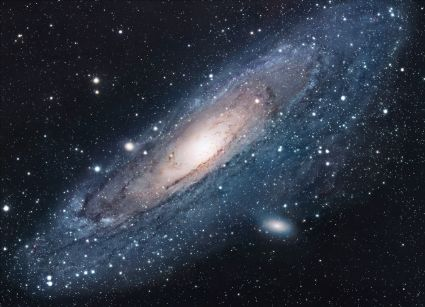
\includegraphics[scale=1.7]{universe}
\caption{The Universe}
\label{fig:universe}
\end{figure}

\section{Conclusion}
``I always thought something was fundamentally wrong with the universe'' \citep{adams1995hitchhiker}

\section{jadval}
\begin{table}[h]
    \begin{center}
     \begin{tabular}{|c|c|c|}
       \hline
       \textbf{A} & \textbf{B} \\
       \hline
        1 & 4  \\
       \hline
       2 & 5  \\
       \hline
       3 & 6 \\
       \hline
     \end{tabular}
     \end{center}
\end{table}


\section{Formool}
\(x + y = M\)



\section{Code}
\begin{lstlisting}[language=C]
fun main (){
    print ("hi !")
}
\end{lstlisting}


\bibliographystyle{plain}
\bibliography{references}
\end{document}
